% Options for packages loaded elsewhere
\PassOptionsToPackage{unicode}{hyperref}
\PassOptionsToPackage{hyphens}{url}
%
\documentclass[
  ignorenonframetext,
]{beamer}
\usepackage{pgfpages}
\setbeamertemplate{caption}[numbered]
\setbeamertemplate{caption label separator}{: }
\setbeamercolor{caption name}{fg=normal text.fg}
\beamertemplatenavigationsymbolsempty
% Prevent slide breaks in the middle of a paragraph
\widowpenalties 1 10000
\raggedbottom
\setbeamertemplate{part page}{
  \centering
  \begin{beamercolorbox}[sep=16pt,center]{part title}
    \usebeamerfont{part title}\insertpart\par
  \end{beamercolorbox}
}
\setbeamertemplate{section page}{
  \centering
  \begin{beamercolorbox}[sep=12pt,center]{part title}
    \usebeamerfont{section title}\insertsection\par
  \end{beamercolorbox}
}
\setbeamertemplate{subsection page}{
  \centering
  \begin{beamercolorbox}[sep=8pt,center]{part title}
    \usebeamerfont{subsection title}\insertsubsection\par
  \end{beamercolorbox}
}
\AtBeginPart{
  \frame{\partpage}
}
\AtBeginSection{
  \ifbibliography
  \else
    \frame{\sectionpage}
  \fi
}
\AtBeginSubsection{
  \frame{\subsectionpage}
}
\usepackage{amsmath,amssymb}
\usepackage{iftex}
\ifPDFTeX
  \usepackage[T1]{fontenc}
  \usepackage[utf8]{inputenc}
  \usepackage{textcomp} % provide euro and other symbols
\else % if luatex or xetex
  \usepackage{unicode-math} % this also loads fontspec
  \defaultfontfeatures{Scale=MatchLowercase}
  \defaultfontfeatures[\rmfamily]{Ligatures=TeX,Scale=1}
\fi
\usepackage{lmodern}
\ifPDFTeX\else
  % xetex/luatex font selection
\fi
% Use upquote if available, for straight quotes in verbatim environments
\IfFileExists{upquote.sty}{\usepackage{upquote}}{}
\IfFileExists{microtype.sty}{% use microtype if available
  \usepackage[]{microtype}
  \UseMicrotypeSet[protrusion]{basicmath} % disable protrusion for tt fonts
}{}
\makeatletter
\@ifundefined{KOMAClassName}{% if non-KOMA class
  \IfFileExists{parskip.sty}{%
    \usepackage{parskip}
  }{% else
    \setlength{\parindent}{0pt}
    \setlength{\parskip}{6pt plus 2pt minus 1pt}}
}{% if KOMA class
  \KOMAoptions{parskip=half}}
\makeatother
\usepackage{xcolor}
\newif\ifbibliography
\usepackage{graphicx}
\makeatletter
\def\maxwidth{\ifdim\Gin@nat@width>\linewidth\linewidth\else\Gin@nat@width\fi}
\def\maxheight{\ifdim\Gin@nat@height>\textheight\textheight\else\Gin@nat@height\fi}
\makeatother
% Scale images if necessary, so that they will not overflow the page
% margins by default, and it is still possible to overwrite the defaults
% using explicit options in \includegraphics[width, height, ...]{}
\setkeys{Gin}{width=\maxwidth,height=\maxheight,keepaspectratio}
% Set default figure placement to htbp
\makeatletter
\def\fps@figure{htbp}
\makeatother
\setlength{\emergencystretch}{3em} % prevent overfull lines
\providecommand{\tightlist}{%
  \setlength{\itemsep}{0pt}\setlength{\parskip}{0pt}}
\setcounter{secnumdepth}{-\maxdimen} % remove section numbering
%\usetheme{metropolis}


%\setbeamercolor{normal text}{bg=white}
%\addtobeamertemplate{frametitle}{}{\vspace{-0.5em}} % decrease
%\setbeamersize{text margin left=5mm,text margin right=10mm}
%\usefonttheme[onlymath]{serif}
%\usefonttheme{professionalfonts}
%%%%%%%%%%%%%%%%
% Packages
%%%%%%%%%%%%%%%%

\usepackage{geometry}
\usepackage{graphicx}
\usepackage{amssymb}
\usepackage{amsopn}
\usepackage{cancel}
\usepackage{epstopdf}
\usepackage{amsmath}  	% this permits text in eqnarray among other benefits
\usepackage{url}		% produces hyperlinks
\usepackage{hyperref}	% allows for color usage in tables
\usepackage[english]{babel}
%\usepackage[latin1]{inputenc}
\usepackage{colortbl}	% allows for color usage in tables
\usepackage{multirow}	% allows for rows that span multiple rows in tables
\usepackage{color}		% this package has a variety of color options
\usepackage{xcolor}
\usepackage{pgf}
\usepackage{calc}
\usepackage{ulem}
\usepackage{multicol}
\usepackage{booktabs}
\usepackage{textcomp}
%\usepackage[misc]{ifsym} % for the dice symbol \Cube{}
%\usepackage{txfonts}
%\usepackage{listings}
%\usepackage{tikz}
\usepackage{array}
\usepackage{wasysym}
\usepackage{fancyvrb}

%% change fontsize of R code
\ifdefined\Shaded
\let\oldShaded\Shaded
\let\endoldShaded\endShaded
\renewenvironment{Shaded}{\footnotesize\oldShaded}{\endoldShaded}
\fi
%% change fontsize of output
\let\oldverbatim\verbatim
\let\endoldverbatim\endverbatim
\renewenvironment{verbatim}{\footnotesize\oldverbatim}{\endoldverbatim}

%%%%%%%%%%%%%%%%
% Remove navigation symbols
%%%%%%%%%%%%%%%%

\setbeamertemplate{navigation symbols}{}

\setbeamertemplate{footline}[frame number]

%%%%%%%%%%%%%%%%
% User defined colors
%%%%%%%%%%%%%%%%

\xdefinecolor{oiB}{rgb}{0.22,0.52,0.72}
\definecolor{oiG}{rgb}{.298,.447,.114}
\xdefinecolor{hlblue}{rgb}{0.051,0.65,1}
\xdefinecolor{gray}{rgb}{0.5, 0.5, 0.5}
\xdefinecolor{darkGray}{rgb}{0.3, 0.3, 0.3}
\xdefinecolor{darkerGray}{rgb}{0.2, 0.2, 0.2}
\xdefinecolor{rubineRed}{rgb}{0.89,0,0.30}
\xdefinecolor{irishGreen}{rgb}{0,0.60,0}	
\definecolor{lightGreen}{rgb}{0.387,0.581,0.148}

%%%%%%%%%%%%%%%%
% Template colors
%%%%%%%%%%%%%%%%

%\setbeamercolor*{palette primary}{fg=white,bg= oiB!80!black!90}
%\setbeamercolor*{palette secondary}{fg=black,bg= oiB!80!black}
%\setbeamercolor*{palette tertiary}{fg=white,bg= oiB!80!black!80}
%\setbeamercolor*{palette quaternary}{fg=white,bg= oiB}
%\setbeamercolor{structure}{fg= oiB}
%\setbeamercolor{frametitle}{bg= oiB!90}
%\setbeamertemplate{blocks}[shadow=false]
%\setbeamersize{text margin left=2em,text margin right=2em}

%\setbeamercolor{code body}{bg=gray!20!white!80,fg=black}


%%%%%%%%%%%%%%%%
% Get rid of fancy enumerated list bullets
%%%%%%%%%%%%%%%%

%\setbeamertemplate{enumerate items}[default]

%%%%%%%%%%%%%%%%
% Custom commands
%%%%%%%%%%%%%%%%

\newcommand{\Sum}{\sum\nolimits}
\newcommand{\Hide}[2]{\underline{~~~\onslide<#1>{\alert{#2}}~~~}}
\newcommand{\hide}[2]{\underline{~~\onslide<#1>{\alert{#2}}~~}}
\newcommand{\hid}[2]{\onslide<#1>{\alert{#2}}}
\newcommand{\code}[1]{\textcolor{blue}{\texttt{#1}}}

% red
\newcommand{\red}[1]{\textit{\textcolor{rubineRed}{#1}}}

% pink
\newcommand{\pink}[1]{\textit{\textcolor{rubineRed!90!white!50}{#1}}}

% green
\newcommand{\green}[1]{\textit{\textcolor{irishGreen}{#1}}}

% orange
\newcommand{\orange}[1]{\textit{\textcolor{orange}{#1}}}

% links: webURL, webLin, appLink
\newcommand{\webURL}[1]{\urlstyle{same}{ \textit{\textcolor{darkGray}{\url{#1}}}}}
\newcommand{\webLink}[2]{\href{#1}{\textcolor{darkGray}{{#2}}}}
\newcommand{\appLink}[2]{\href{#1}{\textcolor{white}{{#2}}}}

% mail
\newcommand{\mail}[1]{\href{mailto:#1}{\textit{\textcolor{darkGray}{#1}}}}

% highlighting: hl, hlGr, mathhl
\newcommand{\hl}[1]{\textit{\textcolor{hlblue}{#1}}}
\newcommand{\hlGr}[1]{\textit{\textcolor{lightGreen}{#1}}}
\newcommand{\mathhl}[1]{\textcolor{hlblue}{\ensuremath{#1}}}

% two col: two columns
\newenvironment{twocol}[4]{
\begin{columns}[c]
\column{#1\textwidth}
#3
\column{#2\textwidth}
#4
\end{columns}
}





%%%%%%%%%%%%%%%%
% Change margin
%%%%%%%%%%%%%%%%

\newenvironment{changemargin}[2]{%
\begin{list}{}{%
\setlength{\topsep}{0pt}%
\setlength{\leftmargin}{#1}%
\setlength{\rightmargin}{#2}%
\setlength{\listparindent}{\parindent}%
\setlength{\itemindent}{\parindent}%
\setlength{\parsep}{\parskip}%
}%
\item}{\end{list}}

%%%%%%%%%%%%%%%%
% Footnote
%%%%%%%%%%%%%%%%

\long\def\symbolfootnote[#1]#2{\begingroup%
\def\thefootnote{\fnsymbol{footnote}}\footnote[#1]{#2}\endgroup}

%%%%%%%%%%%%%%%%
% Graphics
%%%%%%%%%%%%%%%%

\DeclareGraphicsRule{.tif}{png}{.png}{`convert #1 `dirname #1`/`basename #1 .tif`.png}



\setbeamercolor{normal text}{bg=white}

\DeclareMathOperator{\var}{var}
\newcommand{\boxmodel}[1]{\begin{array}{|c|}#1\\[2pt]\hline\end{array}}
\newcommand{\BXX}[2]{\begin{array}{|@{\,}c@{\,}|@{\,}c@{\,}|}\hline#1&#2\\[-1pt]\hline\end{array}}
\newcommand{\p}{\mathrm{P}}
\newcommand{\SE}{\mathrm{SE}}
\newcommand{\xbar}{\overline{x}}
\newcommand{\Xbar}{\overline{X}}
\newcommand{\ybar}{\overline{y}}
\newcommand{\Ybar}{\overline{Y}}
\newcommand{\zbar}{\overline{z}}
\newcommand{\Zbar}{\overline{Z}}
\newcommand{\wbar}{\overline{w}}
\newcommand{\Wbar}{\overline{W}}
\newcommand{\vbar}{\overline{v}}
\newcommand{\Vbar}{\overline{V}}
\newcommand{\dbar}{\overline{d}}
\newcommand{\Dbar}{\overline{D}}
\newcommand{\ebar}{\overline{e}}
\newcommand{\ehat}{\widehat{\epsilon}}
\newcommand{\yhat}{\widehat{y}}
\newcommand{\Yhat}{\widehat{Y}}
\newcommand{\bhat}{\widehat{\beta}}
\newcommand{\dl}[1]{\widehat{\delta}_{#1}}
\newcommand{\g}[1]{\widehat{\gamma}_{#1}}
\newcommand{\al}[1]{\widehat{\alpha}_{#1}}
\newcommand{\Bj}{{\beta_j}}
\newcommand{\Bp}{{\beta_p}}
\newcommand{\Bq}{{\beta_q}}
\renewcommand{\b}[1]{\widehat{\beta}_{#1}}
\newcommand{\B}[1]{{\beta}_{#1}}
\newcommand{\BETA}{{\boldsymbol\beta}}
\newcommand{\bp}{\widehat{\beta}_p}
\newcommand{\bq}{\widehat{\beta}_q}
\newcommand{\bj}{\widehat{\beta}_j}
\newcommand{\df}{\mathrm{df}}
\DeclareMathOperator{\VIF}{VIF}
\DeclareMathOperator{\SSE}{SSE}
\DeclareMathOperator{\SST}{SST}
\DeclareMathOperator{\SSR}{SSR}
\DeclareMathOperator{\MSE}{MSE}
\DeclareMathOperator{\MST}{MST}
\DeclareMathOperator{\MSR}{MSR}
\DeclareMathOperator{\RM}{RM}
\DeclareMathOperator{\FM}{FM}
\DeclareMathOperator{\E}{E}
\DeclareMathOperator{\SD}{SD}
\DeclareMathOperator{\se}{se}
\DeclareMathOperator{\cov}{Cov}
\DeclareMathOperator{\corr}{Corr}
\DeclareMathOperator{\cor}{Cor}
\DeclareMathOperator{\Var}{Var}
\DeclareMathOperator{\logit}{logit}
\newcommand{\hsigma}{\widehat{\sigma}}
\newcommand{\betahat}{\widehat{\beta}}
\newcommand{\slide}{<br><br><br><br><br>}
\newcommand{\bbeta}{\boldsymbol{\beta}}
\newcommand{\bX}{\mathbf{X}}
\newcommand{\bY}{\mathbf{Y}}
\newcommand{\bH}{\mathbf{H}}
\newcommand{\bI}{\mathbf{I}}
\newcommand{\be}{\mathbf{e}}
\newcommand{\pval}{\mathit{P}\mathrm{-val}}



\newcommand{\vmu}{\mbox{\boldmath{$\mu$}}}
\newcommand{\vR}{\mbox{\boldmath{$R$}}}
\newcommand{\vpsi}{\mbox{\boldmath{$\psi$}}}
\newcommand{\vZ}{\mbox{\boldmath{$Z$}}}
\newcommand{\vX}{\mbox{\boldmath{$X$}}}
\newcommand{\vY}{\mbox{\boldmath{$Y$}}}
\newcommand{\vW}{\mbox{\boldmath{$W$}}}
\newcommand{\vz}{\mbox{\boldmath{$z$}}}
\newcommand{\vr}{\mbox{\boldmath{$r$}}}
\newcommand{\vx}{\mbox{\boldmath{$x$}}}
\newcommand{\vk}{\mbox{\boldmath{$k$}}}
\newcommand{\vp}{\mbox{\boldmath{$p$}}}
\newcommand{\vv}{\mbox{\boldmath{$v$}}}
\newcommand{\vg}{\mbox{\boldmath{$g$}}}
\newcommand{\vbeta}{\mbox{\boldmath{$\beta$}}}
\newcommand{\vone}{\mbox{\boldmath{$1$}}}
\newcommand{\vep}{\mbox{\boldmath{$\epsilon$}}}
\newcommand{\veta}{\mbox{\boldmath{$\eta$}}}
\newcommand{\vl}{\mbox{\boldmath{$l$}}}
\newcommand{\ve}{\mbox{\boldmath{$e$}}}
\newcommand{\va}{\mbox{\boldmath{$a$}}}
\newcommand{\vb}{\mbox{\boldmath{$b$}}}
\newcommand{\vPsi}{\mbox{\boldmath{$\Psi$}}}
\DeclareMathOperator*{\V}{\mathbb{V}}


% geometry: topsep=0pt 
\ifLuaTeX
  \usepackage{selnolig}  % disable illegal ligatures
\fi
\IfFileExists{bookmark.sty}{\usepackage{bookmark}}{\usepackage{hyperref}}
\IfFileExists{xurl.sty}{\usepackage{xurl}}{} % add URL line breaks if available
\urlstyle{same}
\hypersetup{
  pdftitle={STAT 20000 Chapter 8Scatterplots \& Correlation},
  hidelinks,
  pdfcreator={LaTeX via pandoc}}

\title{STAT 20000 Chapter 8\newline Scatterplots \& Correlation}
\author{}
\date{\vspace{-2.5em}}

\begin{document}
\frame{\titlepage}

\begin{frame}{How to Draw A Scatter Diagram}
\protect\hypertarget{how-to-draw-a-scatter-diagram}{}
\small

2010 Mean Math SAT Scores\footnote{Source: CollegeBoard} \medskip

\begin{tabular}{c@{}c@{}c}\hline
& {\small Participation} &\\[-3pt]
State & Rate\footnote{The percentage of high school graduates in 2010 that took SAT}
 & Math\\
\hline
AK & 48 & 515\\
AL &  7 & 550\\
AR &  4 & 566\\
AZ & 25 & 525\\
CA & 50 & 516\\
\multicolumn{3}{c}{$\vdots$}\\
IL &  6 & 600\\
\multicolumn{3}{c}{$\vdots$}\\
WY &  5 & 567\\
\hline
\end{tabular}

\vspace{-2.5in}

\begin{flushright}
\includegraphics[width=0.55\linewidth]{ch08_24spr_files/figure-beamer/unnamed-chunk-1-1} \end{flushright}
\end{frame}

\begin{frame}{}
\protect\hypertarget{section}{}
\begin{center}
\includegraphics[width=1\linewidth]{ch08_24spr_files/figure-beamer/unnamed-chunk-2-1} \end{center}
\end{frame}

\begin{frame}{}
\protect\hypertarget{section-1}{}
\begin{center}
\includegraphics[width=1\linewidth]{ch08_24spr_files/figure-beamer/unnamed-chunk-3-1} \end{center}
\end{frame}

\begin{frame}{}
\protect\hypertarget{section-2}{}
One can get the histograms of individual variables from a scatter
diagram.

\vspace{-10pt}

\begin{center}
\includegraphics[width=1\linewidth]{ch08_24spr_files/figure-beamer/unnamed-chunk-4-1} \end{center}
\end{frame}

\begin{frame}{Summarizing a Scatter Diagram}
\protect\hypertarget{summarizing-a-scatter-diagram}{}
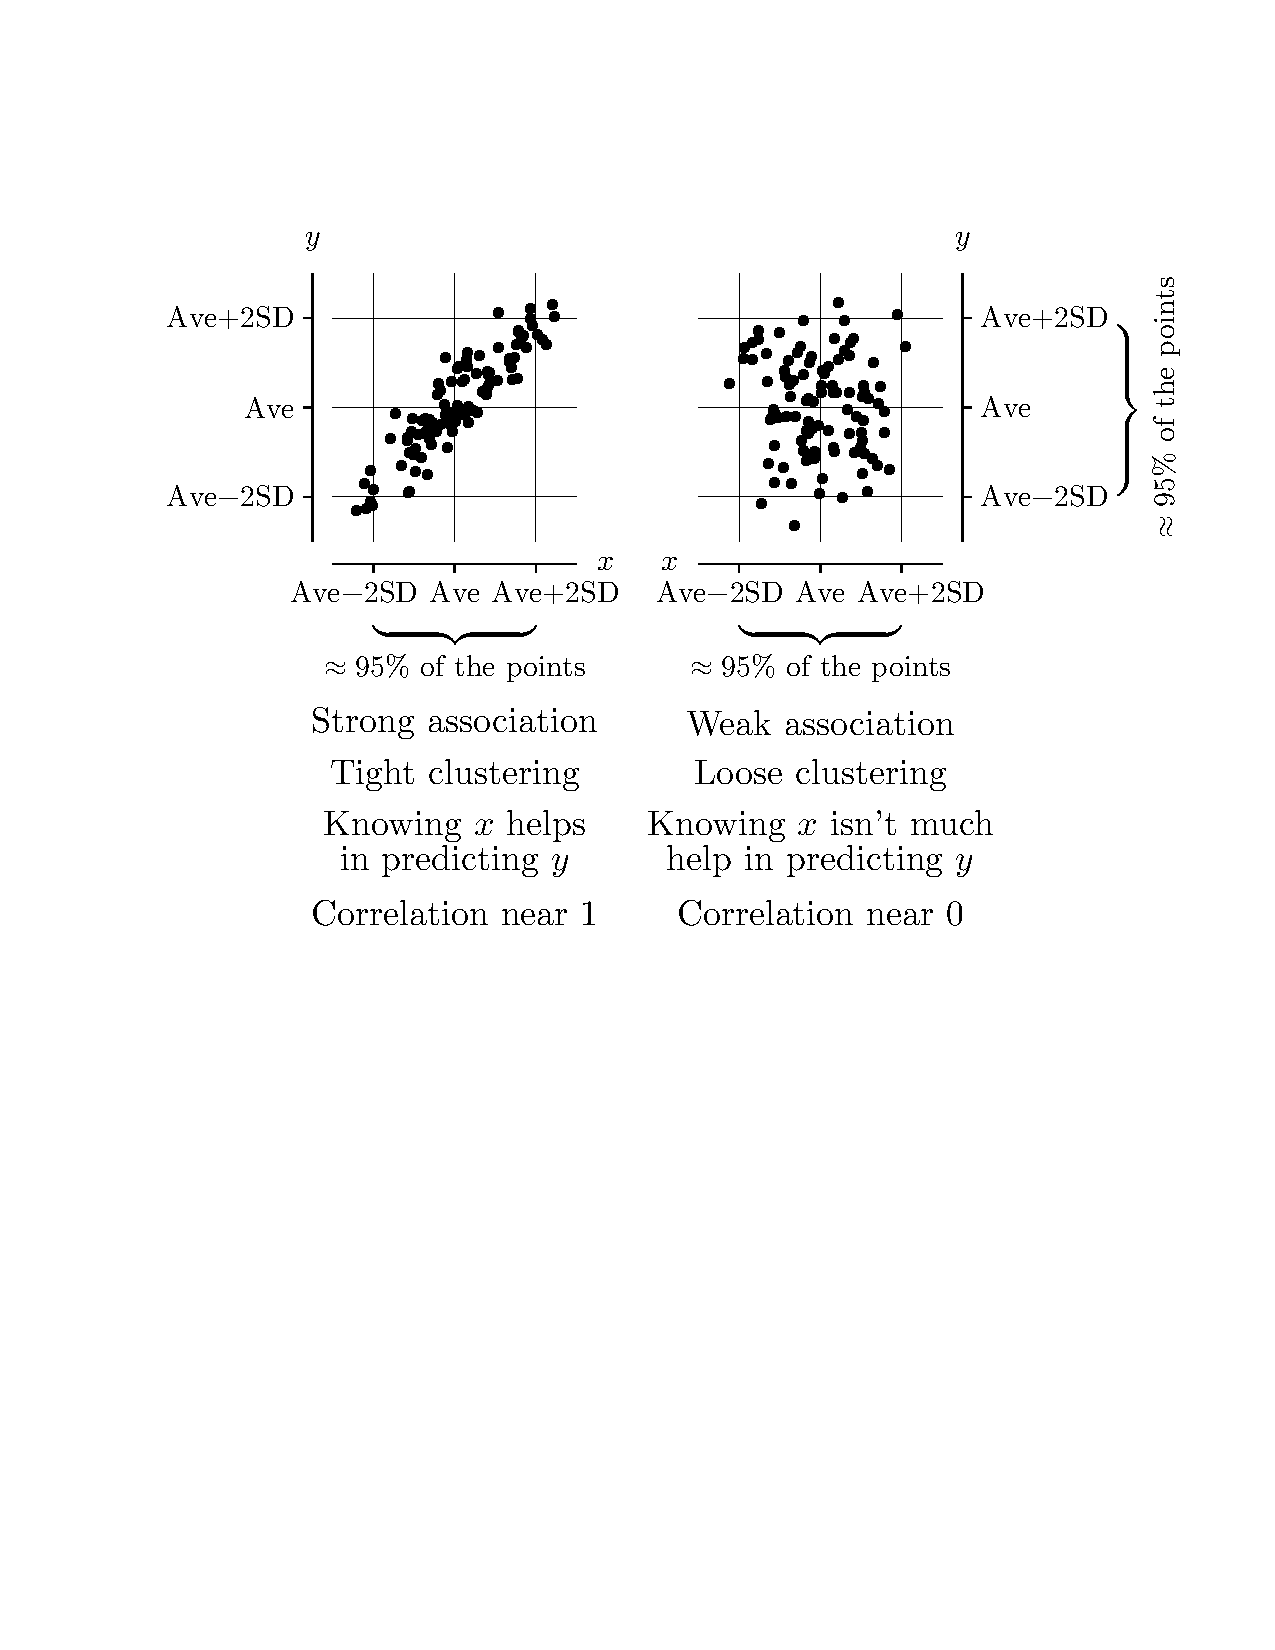
\includegraphics[width=\textwidth]{./C08/ScatterSum.pdf}
\end{frame}

\begin{frame}{Summarizing a Scatter Diagram (Cont'd)}
\protect\hypertarget{summarizing-a-scatter-diagram-contd}{}
A histogram can be summarized by

\begin{itemize}
\tightlist
\item
  average --- center
\item
  SD --- spread
\end{itemize}

A scatter diagram can be summarized by 5 statistics:

\begin{itemize}
\tightlist
\item
  The average and SD of the \(x\)-values
\item
  The average and SD of the \(y\)-values
\item
  The correlation coefficient \(r\)
\end{itemize}

The averages and the SDs specify the center and spread of the cloud of
points, horizontally and vertically. The \(r\) measures the amount of
linear association, i.e., clustering about a line
\end{frame}

\begin{frame}{Forms of Relationship}
\protect\hypertarget{forms-of-relationship}{}

\includegraphics{ch08_24spr_files/figure-beamer/unnamed-chunk-5-1.png}
\end{frame}

\begin{frame}{Positive and Negative Associations}
\protect\hypertarget{positive-and-negative-associations}{}
\(\displaystyle{ \begin{array}{c} \text{Positive}\\[-3pt] \text{Negative} \end{array}}\)
association: High values of one variable tend to occur together with
\(\displaystyle{ \begin{array}{c} \text{high}\\[-3pt] \text{low} \end{array}}\)
values of the other variable.


\includegraphics{ch08_24spr_files/figure-beamer/unnamed-chunk-6-1.png}
\end{frame}

\begin{frame}{Strength of Association}
\protect\hypertarget{strength-of-association}{}
The \textbf{strength} of the relationship between the two variables can
be seen by how much variation, or \textbf{scatter}, there is around the
main form.

\vspace{-4pt}


\includegraphics[width=1\linewidth]{ch08_24spr_files/figure-beamer/unnamed-chunk-7-1}

\vspace{-8pt}
\tabcolsep=0.5in
\begin{tabular}{cc}
Small spread of $Y$ & Large spread of $Y$ \\[-3pt]
 when $X$ is known &  when $X$ is known
\end{tabular}
\end{frame}

\begin{frame}{Clusters \& Outliers}
\protect\hypertarget{clusters-outliers}{}
Sometimes points in a scatter plot form \hl{clusters}, which indicates
data may be comprised of \emph{several distinct kinds of individuals}.

\begin{center}
\includegraphics[width=0.25\linewidth]{ch08_24spr_files/figure-beamer/unnamed-chunk-8-1} \end{center}

Scatter plots can also be used to spot \hl{outliers}.

\begin{center}
\includegraphics[width=0.25\linewidth]{ch08_24spr_files/figure-beamer/unnamed-chunk-9-1} \end{center}
\end{frame}

\begin{frame}{Recap: What to Look For in a Scatterplot?}
\protect\hypertarget{recap-what-to-look-for-in-a-scatterplot}{}
\begin{itemize}[<+->]
\item What is the \hl{form} of the relationship?\\
{\small(linear, curved, clustered ...)}
\item What is the \hl{direction} of the relationship?\\
{\small (positive, negative)}
\item What is the \hl{strength} of the relationship?\\
{\small (strong, weak, ... )}
\item Are the points \hl{clustered}?
\item Are there any deviations from the overall pattern, i.e. \hl{outliers}?
\item In fact, the list above is not exclusive.\\
Any unusual pattern worth investigation.
\end{itemize}
\end{frame}

\begin{frame}{Correlation = Correlation Coefficient, \(r\)}
\protect\hypertarget{correlation-correlation-coefficient-r}{}
\linespread{1}

\hl{Correlation} \(r\) is a numerical measure of the \textbf{direction}
and \textbf{strength} of the \textbf{linear} relationship between two
numerical variables.

``\(r\)'' always lies between \(-1\) and 1; the strength increases as
you move away from 0 to either \(-1\) or 1.

\begin{itemize}
\tightlist
\item
  \(r > 0\): positive association
\item
  \(r < 0\): negative association
\item
  \(r \approx 0\): very weak linear relationship
\item
  large \(|r|\): strong linear relationship
\item
  \(r=-1\) or \(r=1\): \textit{only} when all the data points on the
  scatterplot lie exactly along a \hl{straight line}
\end{itemize}

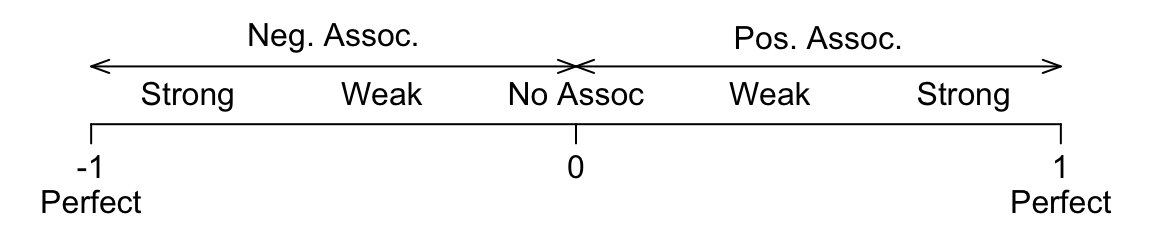
\includegraphics[width=1\linewidth]{ch08_24spr_files/figure-beamer/CorIntro-1}
\end{frame}

\begin{frame}{Positive Correlations}
\protect\hypertarget{positive-correlations}{}
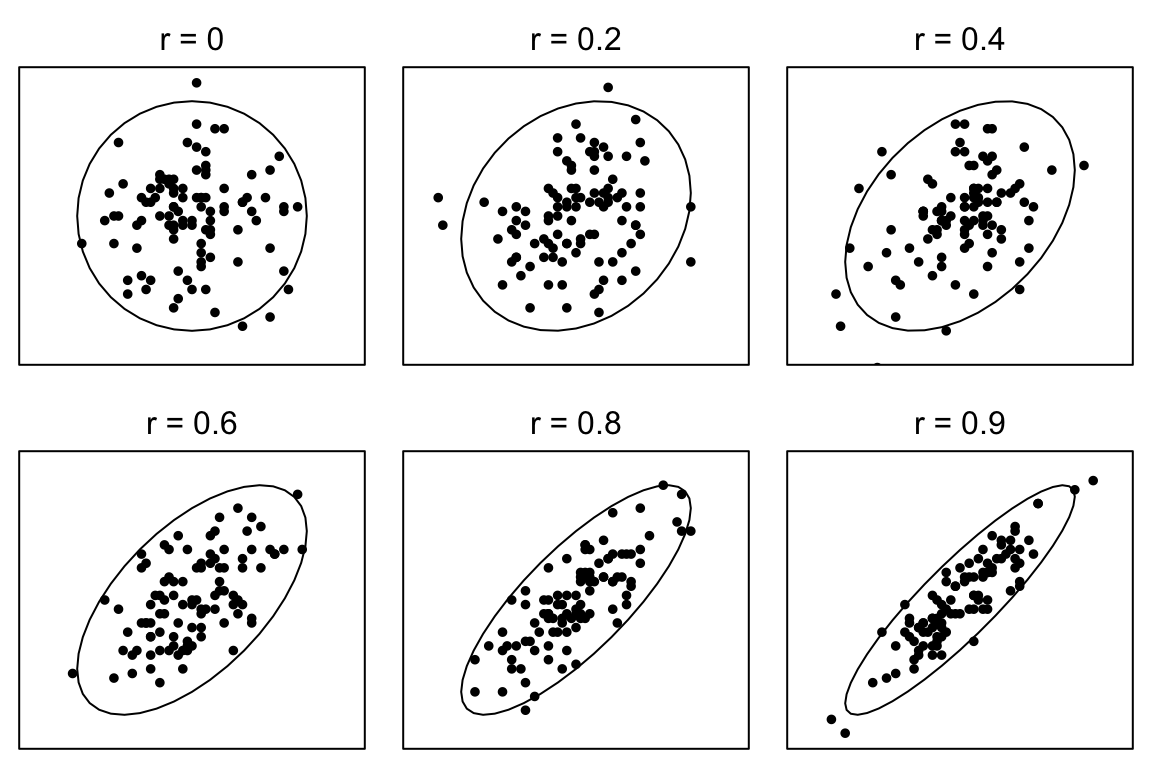
\includegraphics{ch08_24spr_files/figure-beamer/CorPosOval-1.png}
\end{frame}

\begin{frame}{Negative Correlations}
\protect\hypertarget{negative-correlations}{}
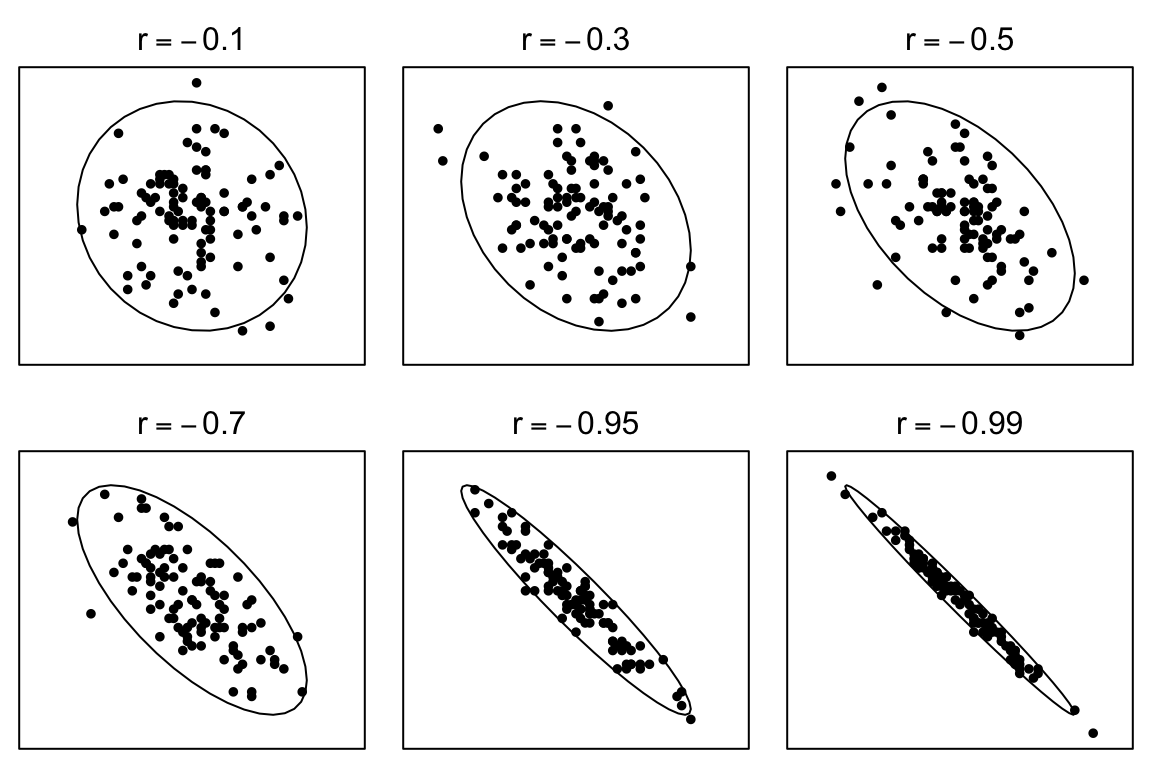
\includegraphics{ch08_24spr_files/figure-beamer/CorNegOval-1.png}
\end{frame}

\begin{frame}{Exercises: Guess \(r\) by Eye}
\protect\hypertarget{exercises-guess-r-by-eye}{}
Match the scatterplots below with the correlation coefficients.
\vspace{-4pt} \[-0.93,\enspace -0.75,\enspace -0.20,\enspace 0.27,
\enspace 0.63, \enspace {\rm and}\enspace 1.0\] \vspace{-20pt}
\only<1| handout:0>{


\begin{center}
\includegraphics[width=0.95\linewidth]{ch08_24spr_files/figure-beamer/unnamed-chunk-10-1} \end{center}


}\only<2| handout:1>{


\begin{center}
\includegraphics[width=0.95\linewidth]{ch08_24spr_files/figure-beamer/unnamed-chunk-10-2} \end{center}


}
\end{frame}

\begin{frame}{Computation of the Correlation Coefficient (r)}
\protect\hypertarget{computation-of-the-correlation-coefficient-r}{}
\begin{columns}[T]
\begin{column}{.18\textwidth}
\begin{align*}
(x_1,\;&y_1)\\
(x_2,\;&y_2)\\
(x_3,\;&y_3)\\
\vdots&\\
(x_n,\;&y_n)
\end{align*}
\end{column}\hspace{-10pt}
\begin{column}{.78\textwidth}
\begin{align*}
r &= \frac{1}{n}\sum_i\left(\frac{x_i-\bar{x}}{\text{SD}_x}\right)\left(\frac{y_i-\bar{y}}{\text{SD}_y}\right)\\
  &= \text{Ave. of ($x$ in standard units) $\times$($y$ in standard units).}
\end{align*}
That is
\begin{itemize}
\item convert each $x$-value and $y$-value into standard units
\item multiply
\item average the product
\end{itemize}
\end{column}
\end{columns}
\end{frame}

\begin{frame}{Why \(r\) Measures the \textcolor{red}{Direction} of a
Linear Relation?}
\protect\hypertarget{why-r-measures-the-of-a-linear-relation}{}
What is the sign of \((x_i-\bar{x})(y_i-\bar{y})\)?

\begin{center}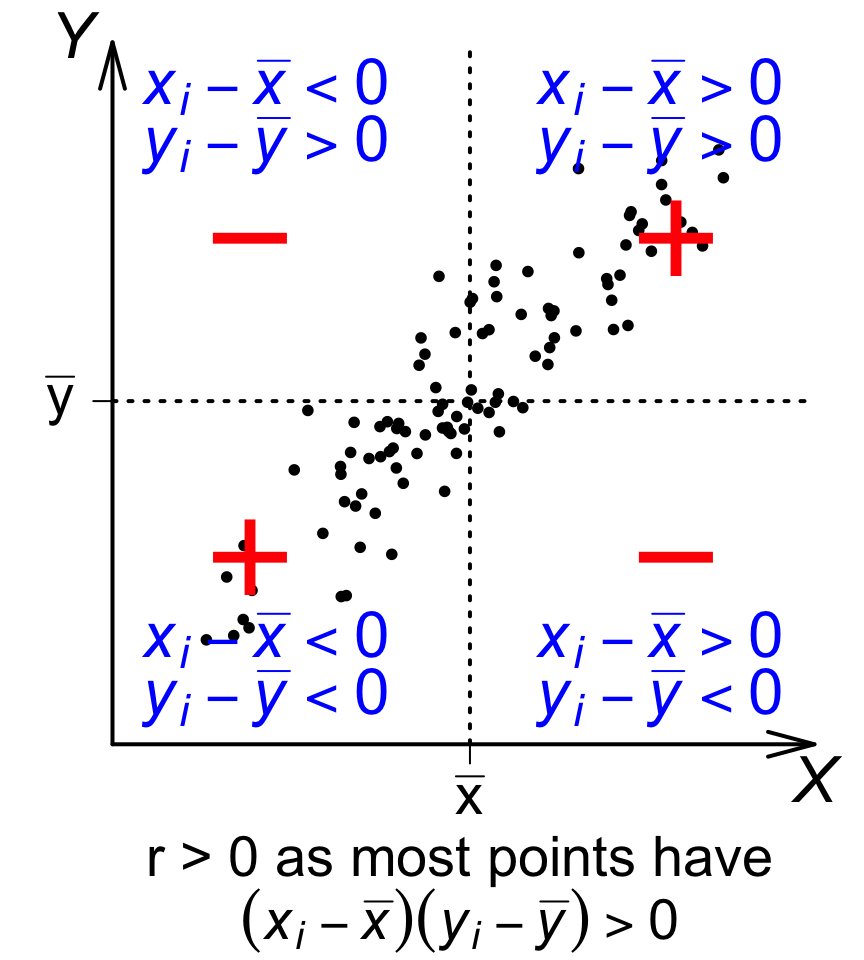
\includegraphics[width=0.49\linewidth]{ch08_24spr_files/figure-beamer/CovDirection-1} 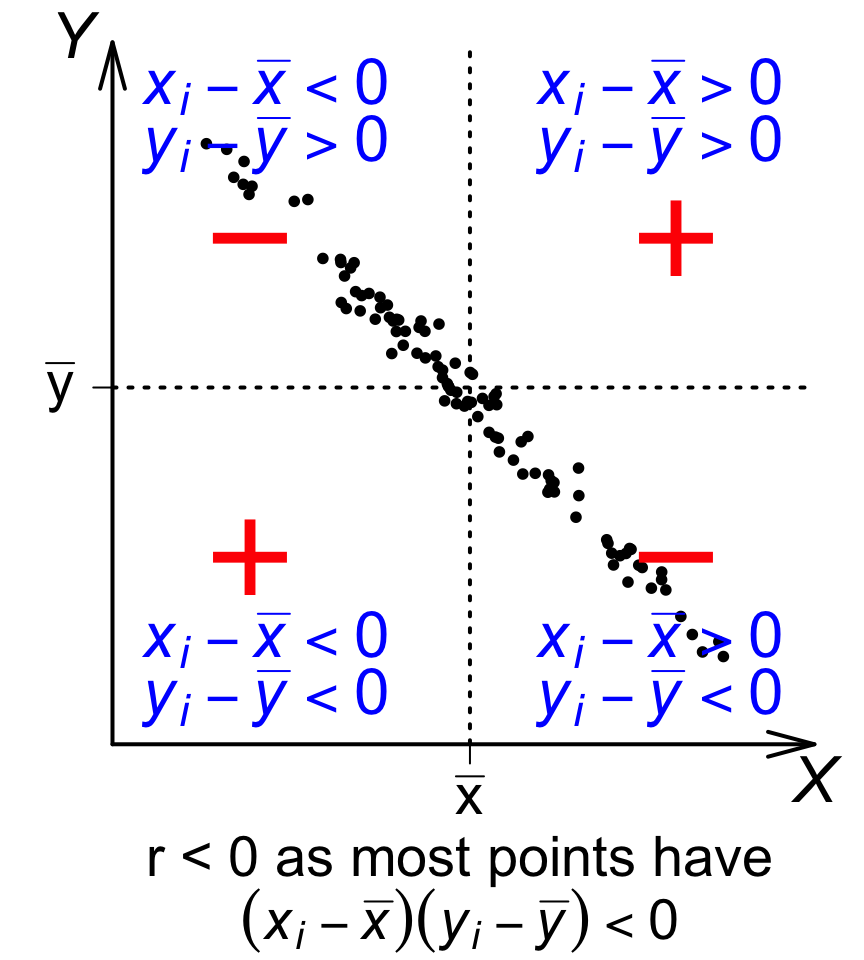
\includegraphics[width=0.49\linewidth]{ch08_24spr_files/figure-beamer/CovDirection-2} \end{center}
\end{frame}

\begin{frame}{Why \(r\) Measures the \textcolor{red}{Strength} of a
Linear Relation?}
\protect\hypertarget{why-r-measures-the-of-a-linear-relation-1}{}
\begin{center}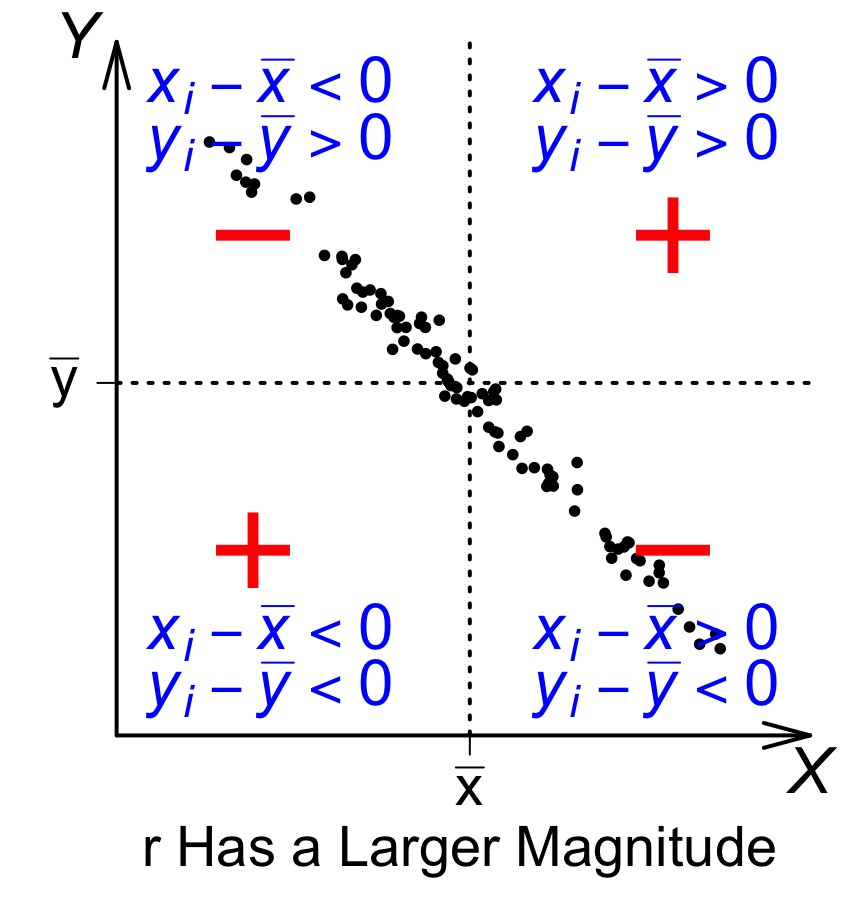
\includegraphics[width=0.49\linewidth]{ch08_24spr_files/figure-beamer/CovStrength-1} 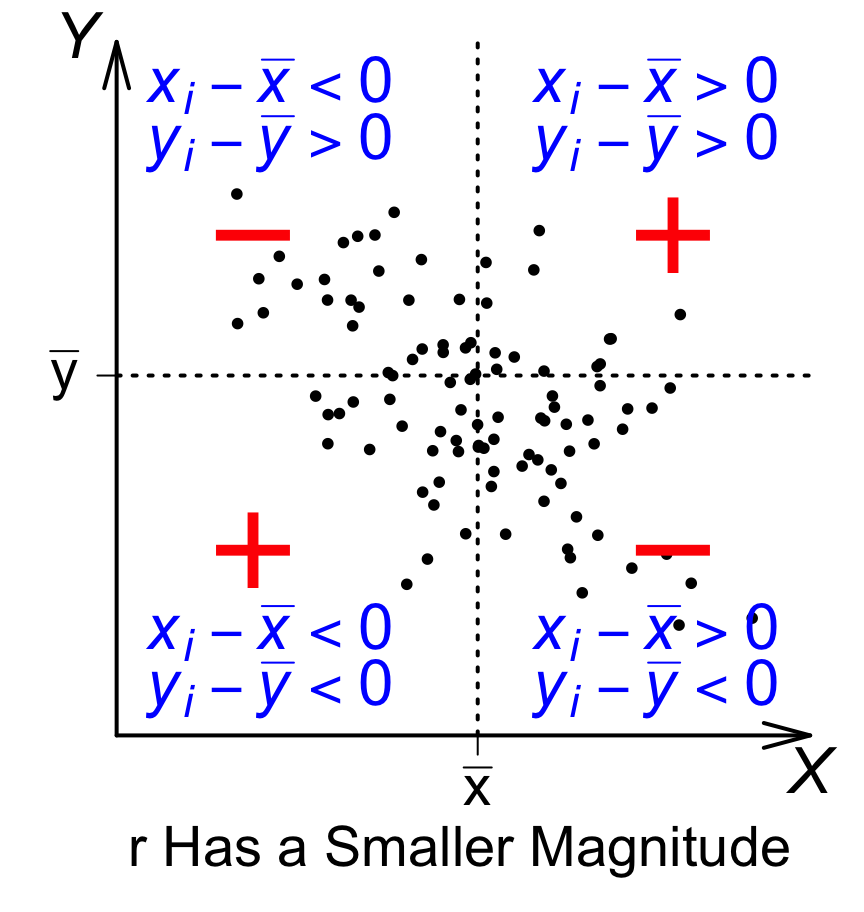
\includegraphics[width=0.49\linewidth]{ch08_24spr_files/figure-beamer/CovStrength-2} \end{center}
\end{frame}

\begin{frame}{Exercise: Computing the Correlation Coefficient}
\protect\hypertarget{exercise-computing-the-correlation-coefficient}{}
A TA gives a quiz with 10 questions to 5 students. The results are:

\begin{center}
\begin{tabular}{cc}
Number right ($x$) & Number wrong ($y$)\\
10 & 0 \\
~8 & 2 \\
~7 & 3 \\
~6 & 4 \\
~4 & 6 \\
\end{tabular}
\end{center}

What is the correlation coefficient?
\end{frame}

\begin{frame}{}
\protect\hypertarget{section-3}{}
\[\boxed{r = \text{Ave. of (SU}_x \times \text{SU}_y)}\] \smallskip

\hrule

\[
\bar{x}=7,\ \text{SD}_x=2,\;
\bar{y}=3,\ \text{SD}_y=2
\] \[
\begin{array}{ccc|ccc|c}
x_i & x_i-\bar{x} & \text{SU}_x & y_i & y_i-\bar{y} & \text{SU}_y & \text{product} \\\hline
 10 &  ~3 &  3/2 & 0 & -3 & -3/2& -9/4\\ ~8 &  ~1 &  1/2 & 2 & -1 & -1/2& -1/4\\
 ~7 &  ~0 &  0   & 3 &  0 & 0   &  0  \\
 ~6 &  -1 & -1/2 & 4 &  1 &  1/2& -1/4\\
 ~4 &  -3 & -3/2 & 6 &  3 &  3/2& -9/4\\
\end{array}
\] \[
r =
\begin{array}{c} \text{average of}\cr \text{product}\end{array}
  = \frac{1}{5}\left( \frac{-9 -1 +0 -1 -9}{4} \right) =
\frac{-20}{20} = -1
\] Is there an easier way to reach this conclusion?

\hid{2-}{Yes, all points lie on a downward sloping straight line
$$\text{Number wrong}  = 10 - \text{Number right}$$
Thus, $r$ must be~$-1$.}
\end{frame}

\end{document}
